% BALL IDENTIFICATION REPORT
% by Marco Giacomin

\section{Ball Identification}

The task of ball identification is as such: 
given a precise window inside an image that is assumed to 
contain a ball of the game of pool, we want to identify 
which type it belongs to (whether cueball, 8-ball, striped or 
solid color). We assume we don't need to identify the precise 
number of the ball outside of the number 8 one.

The main insight into this task is the fact that the most 
identifying element of a ball is its amount of white paint. 
A cueball is completely covered in it, a striped ball is 
covered about halfway and a solid or 8-ball has only a small 
white circle around its number. If we can find a way to 
reliably count the proportion of white pixels in the ball area 
and a corresponding expected range associated with each class 
the remaining task will only be one of distinguishing the 
8-ball from the other solid color balls.

The main challenges of this sub-task are:
\begin{enumerate}
  \item ensuring robustness to illumination changes
  \item coping with specific ball color 
  (some of them might be of a brightness approaching white)
\end{enumerate}

A typical input image will look like this:
\begin{figure}[h]
  \centering
  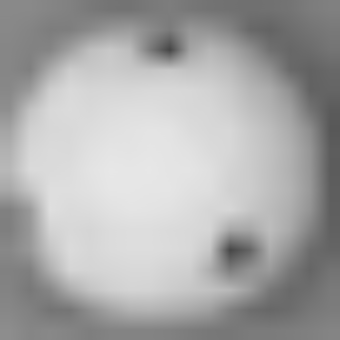
\includegraphics[width=0.4\textwidth]{./imgs/cueball_grey.png}
  \caption{Grayscale image of a cueball}
\end{figure}

\begin{figure}[h]
  \centering
  
\includegraphics[width=0.4\textwidth]{./imgs/difficult_solid.png}
  \caption{Grayscale image of a solid ball}
\end{figure}

My first approach was to attempt Otsu thresholding segmentation
on a grayscale version of the ball image, 
via the built-in \verb|THRESH_OTSU| option in the \verb|threshold| function.
Unfortunately this produced a very inconsistent separation between white and 
colored pixels which only sometimes corresponded to a real white region 
on the image, especially for images of solid colored balls.

\begin{figure}[h]
  \centering
  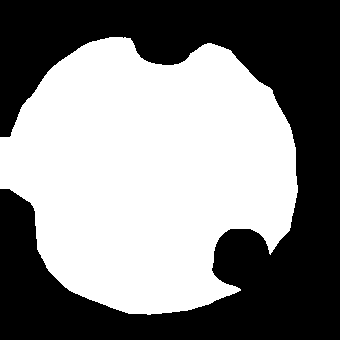
\includegraphics[width=0.4\textwidth]{./imgs/cueball_otsu.png}
  \caption{Otsu segmentation of a cueball}
\end{figure}

\begin{figure}[h]
  \centering
  
\includegraphics[width=0.4\textwidth]{./imgs/bad_otsu.png}
  \caption{Failed otsu segmentation of a solid ball}
\end{figure}

My second attempt involved color-space clustering via \verb|kmeans|. 
The underlying intuition is as such: a well-cropped window of a ball should 
contain roughly three important areas of uniform color: the table cloth and 
the colored and white parts on the surface of the ball. This means that 
we could theoretically employ a clustering algorithm on the color space 
of the pixels to separate these areas and count how many respective pixels 
appear per each type in the image.  
Unfortunately, this type of segmentatation performed even worse than the 
previous one due to illumination effects that cast pixels of one class 
into another.

A possible way to counteract this would be to factor in radial distance 
from the estimated ball center to the feature space of the clustering, 
which would at least help differentiate the pixels belonging to the 
ball from the ones belonging to the cloth. However, I didn't attempt 
this because I found a method that proved to be significantly more 
performand than the previous two:

The third approach consists in a simple thresholding and white pixel 
counting, with the difference that the image is first set to zero 
outside of the inscripted ellipse (the approximate location of the ball)
to avoid false positives in the surrounding area and the grayscale 
intensity of the remaining pixels is stretched to occupy the full 
0-255 range. A relative threshold (chosen on the basis of the example 
data) is then applied and the ball type is decided based on the 
percentage of white pixels remaining.

\begin{figure}[h]
  \centering
  
\includegraphics[width=0.4\textwidth]{./imgs/difficult_solid_identified.png}
  \caption{Correctly segmented white part of a solid ball}
\end{figure}

Unfortunately, this method produces some incorrect classifications 
and cannot distinguish between a solid color ball and an 8-ball. 
While the first problem would require a more sophisticate approach 
(possibly a machine learning one if sufficient performance is 
required), the second is solvable by building a higher level 
classification method: the function \verb|classifyBalls| takes 
in the whole image, plus a vector of windows that correspond to 
the predicted balls locations. 
The function isolates the brightest and darkest windows, which 
get labeled respectively as the cueball and the 8-ball. 
The remaining windows are then handled singularly using the previously 
defined approach.